%!TEX TS-program = xelatex
\documentclass[]{friggeri-cv}
\usepackage{afterpage}
\usepackage{hyperref}
\usepackage{color}
\usepackage{xcolor}
\hypersetup{
    pdftitle={},
    pdfauthor={},
    pdfsubject={},
    pdfkeywords={},
    colorlinks=false,       % no lik border color
   allbordercolors=white    % white border color for all
}
\addbibresource{bibliography.bib}
\RequirePackage{xcolor}
\definecolor{pblue}{HTML}{0395DE}

\begin{document}
\header{Prashant} {Tiwari}
      {Backend Developer}
      
% Fake text to add separator      
\fcolorbox{white}{gray}{\parbox{\dimexpr\textwidth-2\fboxsep-2\fboxrule}{%
.....
}}

% In the aside, each new line forces a line break
\begin{aside}
  \section{Address}
    97, Western Road,
    E13 9JE, London, UK
    ~
  \section{Twitter}
    \href{https://twitter.com/tintin5us}{\textbf{@tintin5us}}
    ~
  \section{Skype}
    prashanttiwari247
    ~
  \section{Mail}
    \href{mailto:prashanttiwari247@gmail.com}{\textbf{prashanttiwari247@}\\gmail.com}
    ~
  \section{Web \& Git}
    \href{http://www.prashanttiwari.com}{prashanttiwari.com}
    \href{https://github.com/pt247}{github.com/pt247}
    ~
  \section{Programming}
    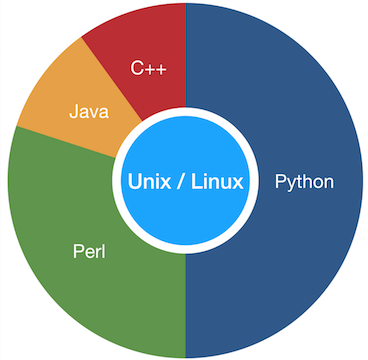
\includegraphics[scale=0.62]{img/programming.png}
    ~
  \section{OS Preference}
    \textbf{GNU/Linux}
\includegraphics[scale=0.40]{img/5stars.png}
    \textbf{Unix}
\includegraphics[scale=0.40]{img/4stars.png}
    \textbf{MacOS}
\includegraphics[scale=0.40]{img/3stars.png}
    ~
  \section{Personal Skills}
    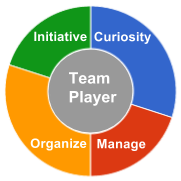
\includegraphics[scale=0.62]{img/personal.png}
    ~
\end{aside}

\section{Experience}
\begin{entrylist}
  \entry
    {12/16 - Now}
    {Lead Backend developer}
    {Powervault, London, UK}
    {Design and implement back-end for internet of things infrastructure that can scale horizontally. Work with a wide range of tools: Django Rest Framework, Flask, Ansible, Influx and MySql, Kafka. Lead a team of 3 Python developers. \\}
  \entry
    {11/15 - 10/16}
    {Computer Scientist}
    {Edgefolio, London, UK}
    {Design, enhance and maintain data acquisition layer for flagship project. Implement comprehensive test coverage and doing TDD where possible. Perform root cause analysis for critical production issues. Tools used: Python, Django REST framework, Pandas, Linux.Working on creating useful incites from user analytics.
    .\\}
    \entry
    {07/15 - 11/15}
    {Freelance Developer \& Consultant}
    {Freelancer.com, UK}
    {Single page Flask application that uses Numpy and Scipy in background to parse OMR sheets (answer papers). Work on small python projects.\\}
    \entry
    {01/09 - 07/15}
    {Team Lead}
    {Persistent, Pune, India}
    {Responsible for back end python programming, I implemented helped implement an ambitious project to automate all terminal side testing across the globe. Design and enhancement of python based test automation framework. Evolve a POC project into a full-fledged functional product in less than 6 months. Pythonic, idiomatic, DRY code to efficiency handle large data streams of logs coming in
    from thousands of terminals (Point of Sales devices) simultaneously using socket programming.\\}
    \entry
    {03/11 - 01/15}
    {Tata Consultancy Services}
    {Consultant at Morgan Stanley, London, UK}
    {Responsible for maintaining 2 million worth of agency flow from algorithmic trading spread across almost all European destinations. Part of European team that specializes in providing high speed algorithmic trading platform. Perl/Python/Shell Integration specialist responsible for client on-boarding, continues integration environment, and all Perl/ Python development. Work with FIX libraries for creating a order flow tool from regular log files. Sole maintainer for Python based object oriented library for parsing configuration files used by various reporting and risk identification tools and for process management. Review and re-factored existing Perl monitoring scripts to reduce 95\% of daily automated
    emails to support groups and helping them better support Speedway. Tools used: Perl, Python, Unix, Sybase}
    \entry
    {11/09 - 02/11}
    {Tata Consultancy Services}
    {Core team member, Mumbai, India}
    {Automate testing for risk assessment engine used by Morgan Stanley. Tools used: Perl\\}
    \entry
    {11/06 - 11/09}
    {Merce Technologies Pvt Ltd.}
    {Consultant at Morgan Stanley, Pune, India}
    {Develop Perl CGI applications for various interfaces and screens for Merce's flagship project. Developed, tested and deployed Perl data acquisition application at all 5 Zodiac factories spread across India as a individual contributor. Socket programming in Perl to communication to terminals. Tools used: Perl\\}
\end{entrylist}

\section{Education}
\begin{entrylist}
  \entry
    {2001 - 2006}
    {Bachelor's Degree in Electrical and Electronics  Engineering}
    {RGPV, Bhopal, India}
    {Main subjects: Electrical and Electronics, Digital Signal Processing, Digital and Analogical Electronics.\\
    }
 
\end{entrylist}

\section{Certifications}
\begin{entrylist}
  \entry
    {2004}
    {SCJP}
    {Oracle}
    {\emph{Sun Certified Java Programmer for version 1.4}}
    
  \entry
    {2015}
    {Introduction to Python for Data Science}
    {edX}
    {\emph{Python for Data Science}}

  \entry
    {2017}
    {Understanding GB Energy Markets}
    {Cronwall Insights}
    {\emph{‘Understanding GB Energy Markets’ training.}}
\end{entrylist}


% \begin{aside}
%~
%~
%~
%  \section{Places Lived}
%    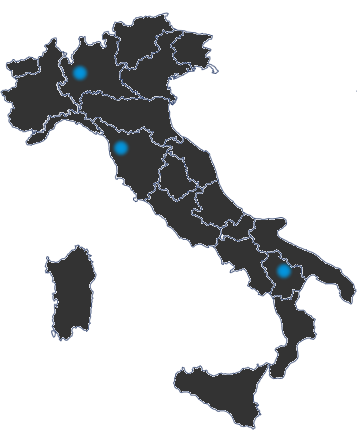
\includegraphics[scale=0.25]{img/italia.png}
%   ~
% \section{Languages}
%   \textbf{Italian}
\includegraphics[scale=0.40]{img/5stars.png%}
%   \textbf{English}
\includegraphics[scale=0.40]{img/4stars.png%}
%\end{aside}


\section{Other Info}
Tools and technologies worked on:\\
\emph{ Python, Perl, Kafka, Jenkins, Git, Jira, socket programming, shell scripting, FIX protocol, Native exchange protocols, application support, RCA, system administration, Unix, testing, Sybase, Mysql, Postgres, Autosys, Front office, Low latency application support.}
\\

Co-organizer PyData London monthly MeetUp and yearly Conference:\\
\href{https://www.meetup.com/PyData-London-Meetup/}{meetup.com/PyData-London-Meetup/}\\
\emph{PyData is an educational program of NumFOCUS, a 501(c)3 non-profit organization in the United States. PyData provides a forum for the international community of users and developers of data analysis tools to share ideas and learn from each other. The global PyData network promotes discussion of best practices, new approaches, and emerging technologies for data management, processing, analytics, and visualization. PyData communities approach data science using many languages, including (but not limited to) Python, Julia, and R.}
\\
\begin{flushleft}
\emph{January 2nd, 2018}
\end{flushleft}
\begin{flushright}
\emph{Prashant Tiwari}
\end{flushright}

\end{document}
